% --- [ Hammock Method ] -------------------------------------------------------

\subsection{Hammock Method}
\label{sec:hammock_method}

The Hammock method is a control flow analysis method which identifies control flow primitives in CFGs based on subgraph isomorphisms. More specifically, a set of high-level control flow primitives may be represented as canonical single-entry single-exit subgraphs\footnote{\textit{One potential reference for the naming of the Hammock method, is that the subgraphs are single-entry single-exist and are thus connected in two end-points, analogous to hammocks.}} (see figure \ref{fig:graph_representations}), and these subgraphs may be identified in CFGs using subgraph isomorphism search algorithms \cite{node_splitting}.

\begin{savenotes}
	\begin{figure}[htbp]
		\centering
		% if
		\begin{subfigure}[ht]{0.23\textwidth}
			\centering
			\begin{subfigure}[ht]{0.45\textwidth}
				\lstinputlisting[language=go, style=go, breaklines=false, numbers=none]{inc/primitives/if.c}
			\end{subfigure}
			\begin{subfigure}[ht]{0.42\textwidth}
				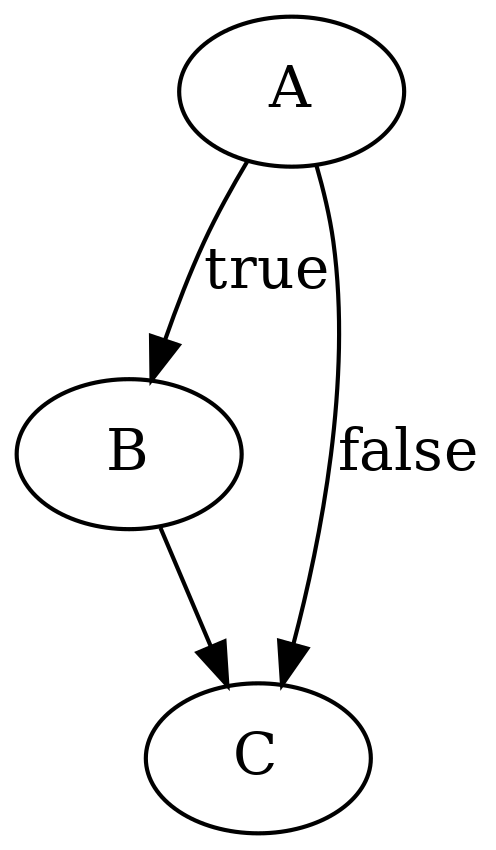
\includegraphics[width=\textwidth]{inc/primitives/if.png}
			\end{subfigure}
			\caption{1-way conditional; entry: \texttt{A}, exit: \texttt{C}.}
			\label{fig:if_graph_representation}
		\end{subfigure}
		\qquad
		% if_else
		\begin{subfigure}[ht]{0.28\textwidth}
			\centering
			\begin{subfigure}[ht]{0.45\textwidth}
				\lstinputlisting[language=go, style=go, breaklines=false, numbers=none]{inc/primitives/if_else.c}
			\end{subfigure}
			\begin{subfigure}[ht]{0.50\textwidth}
				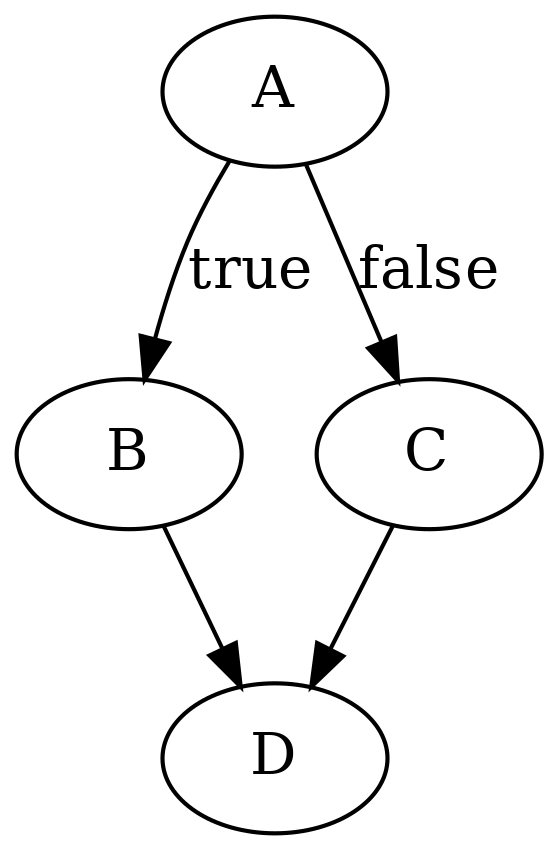
\includegraphics[width=\textwidth]{inc/primitives/if_else.png}
			\end{subfigure}
			\caption{2-way conditional; entry: \texttt{A}, exit: \texttt{D}.}
			\label{fig:if_else_graph_representation}
		\end{subfigure}
		\qquad
		% if_return
		\begin{subfigure}[ht]{0.30\textwidth}
			\centering
			\begin{subfigure}[ht]{0.45\textwidth}
				\lstinputlisting[language=go, style=go, breaklines=false, numbers=none]{inc/primitives/if_return.c}
			\end{subfigure}
			\begin{subfigure}[ht]{0.50\textwidth}
				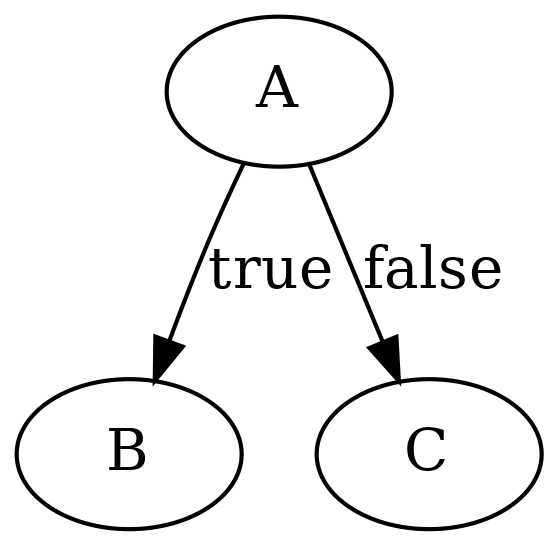
\includegraphics[width=\textwidth]{inc/primitives/if_return.png}
			\end{subfigure}
			\caption{1-way condition with return statement in body; entry: \texttt{A}, exit: \texttt{C}.}
			\label{fig:if_return_graph_representation}
		\end{subfigure}
		\qquad
		% pre_loop
		\begin{subfigure}[ht]{0.32\textwidth}
			\centering
			\begin{subfigure}[ht]{0.45\textwidth}
				\lstinputlisting[language=C, style=go, breaklines=false, numbers=none]{inc/primitives/pre_loop.c}
			\end{subfigure}
			\begin{subfigure}[ht]{0.50\textwidth}
				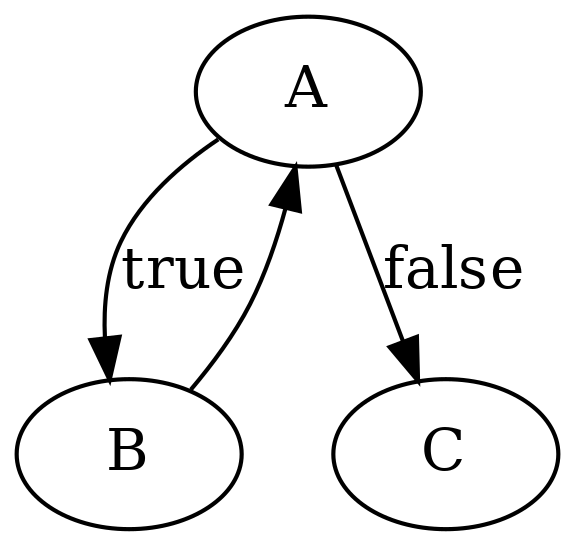
\includegraphics[width=\textwidth]{inc/primitives/pre_loop.png}
			\end{subfigure}
			\caption{pre-test loop; entry: \texttt{A}, exit: \texttt{C}.}
			\label{fig:pre_loop_graph_representation}
		\end{subfigure}
		\qquad
		% post_loop
		\begin{subfigure}[ht]{0.30\textwidth}
			\centering
			\begin{subfigure}[ht]{0.50\textwidth}
				\lstinputlisting[language=C, style=go, breaklines=false, numbers=none]{inc/primitives/post_loop.c}
			\end{subfigure}
			\begin{subfigure}[ht]{0.35\textwidth}
				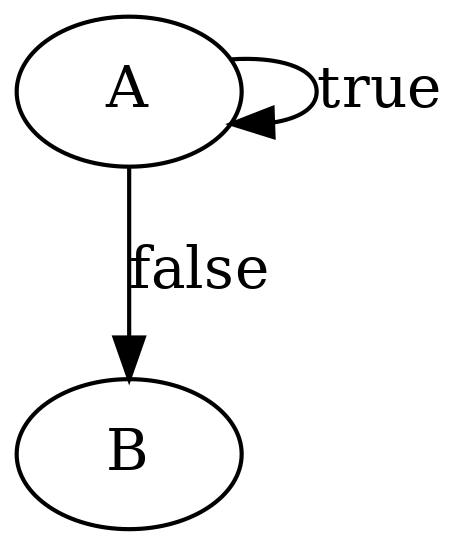
\includegraphics[width=\textwidth]{inc/primitives/post_loop.png}
			\end{subfigure}
			\caption{post-test loop; entry: \texttt{A}, exit: \texttt{B}.}
			\label{fig:post_loop_graph_representation}
		\end{subfigure}
		\qquad
		% seq
		\begin{subfigure}[ht]{0.24\textwidth}
			\centering
			\begin{subfigure}[ht]{0.20\textwidth}
				\lstinputlisting[language=C, style=go, breaklines=false, numbers=none]{inc/primitives/seq.c}
			\end{subfigure}
			\begin{subfigure}[ht]{0.35\textwidth}
				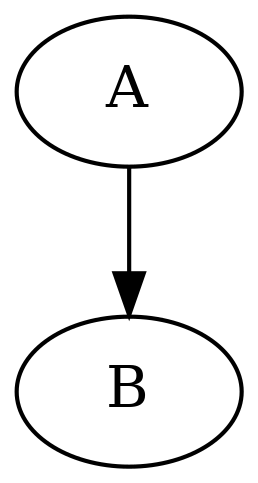
\includegraphics[width=\textwidth]{inc/primitives/seq.png}
			\end{subfigure}
			\caption{consecutive statements; entry: \texttt{A}, exit: \texttt{B}.}
			\label{fig:seq_graph_representation}
		\end{subfigure}
		\caption{The pseudo-code and graph representation of various high-level control flow primitives with denoted entry and exit nodes.\protect\footnote{Note, the Hammock method section is in part adapted from section 2.2.3 (Control Flow Analysis) of \cite{compositional_decompilation}, as written by the same author as this project.}}
		\label{fig:graph_representations}
	\end{figure}
\end{savenotes}

% TODO: rephrase the following paragraph.

To recover nested control flow primitives, the Hammock method iteratively performs subgraph isomorphism search to locate canonical subgraphs of high-level control flow primitives. Once a subgraph has been located, the algorithm merges the nodes of the subgraph into a single node, which has the incoming edges of the entry node and the outgoing edges of the exit node; as illustrated in figure \ref{fig:subgraph_merge}. This process is repeated until either the CFG contains a single node, in which case the CFG was translated to an AST containing only high-level control flow primitives -- or no more subgraph isomorphisms can be located -- in which case \texttt{goto} statements have to be used to describe the CFG.

\begin{figure}[htbp]
	\centering
	\begin{subfigure}[ht]{0.17\textwidth}
		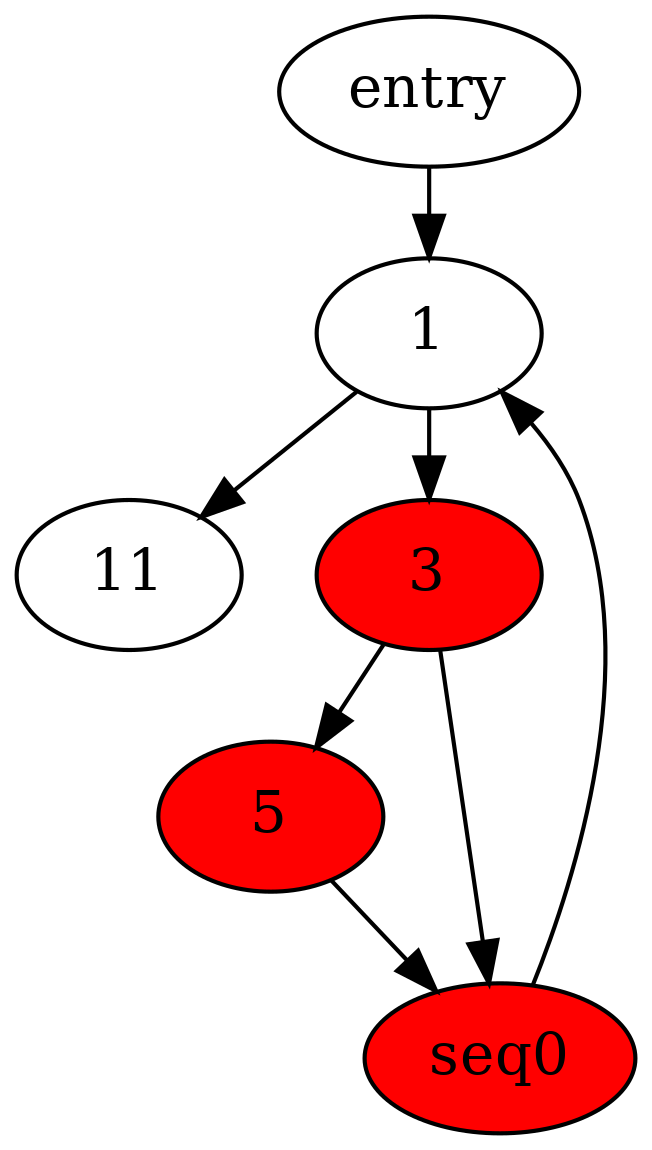
\includegraphics[width=\textwidth]{inc/3_background/hammock_method/cfg_pre_merge.png}
	\end{subfigure}
	\qquad
	\begin{subfigure}[ht]{0.17\textwidth}
		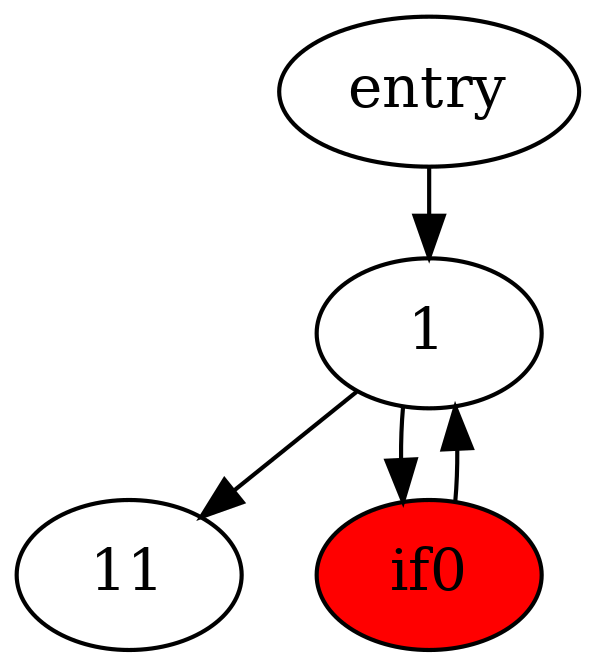
\includegraphics[width=\textwidth]{inc/3_background/hammock_method/cfg_post_merge.png}
	\end{subfigure}
	\caption{The CFG of a function in which the canonical subgraph of a 1-way conditional (see figure~\ref{fig:if_graph_representation}) has been identified (left side), and the same CFG after the subgraph has been replaced with a single node \texttt{if0} that inherits the predecessors of the subgraph entry node \texttt{3} and the successors of the subgraph exit node \texttt{seq0} (right side).}
	\label{fig:subgraph_merge}
\end{figure}

% From Cifuentes'. Not about this paper, but relevant. Lichtblau[Lic85] presented a series of transformation rules to transform a control flow graph into a trivial graph by identifying subgraphs that represent high-level control structures; such as 2-way conditionals, sequence, loops, and multiexit loops. Whenever no rules were applicable to the graph, an edge was removed from the graph and a goto was generated in its place. This transformation system was proved to be finite Church-Rosser, thus the transformations could be applied in any order and the same final answer is reached.

% ---> Important. Notes from Cifuentes'. Not about this paper, but relevant. The detection of control structures by means of graph transformations does not modify the semantics or functionality of the underlying program, thus a transformation system provides a method to generate a semantically equivalent graph.

% TODO: add note that Hammock does not handle compound boolean conditions? I.e. short-circuit.
